\documentclass[12pt]{article}

\usepackage[margin=1in]{geometry}

\usepackage{amsmath, graphicx, caption, subcaption, xcolor}

\graphicspath{{res/}}

% I need a punchy title which is general enough
% to fit all three (if I can pull them off) points from the lab manual.
\title{\textcolor{red}{The Galactic Plane}}

\author{Lukas Finkbeiner}

\begin{document}

\maketitle

%\begin{figure}
%	\centering
%	\includegraphics[width=.6\linewidth]{filename}
%	\caption{}
%	\label{fig: ...}
%\end{figure}

\begin{abstract}

% remember to motivate the paper

We study

1. velocity patterns of various H clouds using Doppler shifts

2. black hole mass

3. accuracy of a spiral arm fit

results, uncertainties.

\end{abstract}

\section{Introduction and Background}


\begin{equation} \label{eq:spiral}
R_\text{arm} = R_0 e^{\kappa(\phi - \phi_0)}
\end{equation}

The following equation is a conclusion of the tangent-point method for converting galactic rotation to Doppler velocity. $R_\odot \approx 220 $ km / s and $R_\odot \approx 8.5$ kpc $\equiv 2.6 \times 10^{17}$ km. 

\begin{equation} \label{eq:vel_dopp}
V_\text{Dopp} = \left[ \frac{V(R)}{R} - \frac{V(R_\odot)}{R_\odot} \right] R_\odot \sin(\ell)
\end{equation}

%\begin{equation}
%\frac{V_\text{Dopp}}{R_\odot \sin \ell} = \frac{V(R)}{R} - \frac{V(R_\odot)}{R_\odot}
%\end{equation}

%\begin{equation}
%\frac{V_\text{Dopp}}{R_\odot \sin \ell} + \frac{V(R_\odot)}{R_\odot} = \frac{V(R)}{R} = \frac{1}{R_\odot} \left[ \frac{V_\text{Dopp}}{\sin \ell} - V(R_\odot) \right] 
%\end{equation}

The following representation will be used in establishing the velocity curve inside the solar circle:

\begin{equation} \label{eq:vel_curve}
V(R) = \frac{R}{R_\odot} \left[ \frac{V_\text{Dopp}}{\sin \ell} - V(R_\odot) \right] 
\end{equation}

This next form will be used in placing points outside the solar circle, to evaluate the spiral shape:

%\begin{equation}
%\frac{V_\text{Dopp}}{R_\odot \sin \ell} = \frac{V(R)}{R} - \frac{V(R_\odot)}{R_\odot}
%\end{equation}

%\begin{equation}
%\frac{V(R)}{R} = \frac{V_\text{Dopp}}{R_\odot \sin \ell} + \frac{V(R_\odot)}{R_\odot} 
%\end{equation}

\begin{equation} \label{eq:outer_spiral}
R = V(R) \left[ \frac{V_\text{Dopp}}{R_\odot \sin \ell} + \frac{V(R_\odot)}{R_\odot} \right]^{-1}
\end{equation}


%\textcolor{red}{You have to cite sources and find a better common unit.}

We also want gain / calibration equations from lab 2.

\begin{equation} \label{eq:line_shape}
T_\text{line} = G \, \frac{s_\text{on}}{s_\text{off}}
\end{equation}

where

\begin{equation} \label{eq:line_gain}
G = \frac{T_\text{sys, cal} - T_\text{sys, cold}}{\sum{(s_\text{cal} - s_\text{cold})}} \sum{s_\text{cold}}
\end{equation}

Given certain patterns, how well does a spiral fit? We need to control for the total number of data. We want the normalization of any two compared sets to be the same (so, we scale accordingly). What numpy functions I used.

21 cm line transition: 1420.405751786 MHz at rest.


\begin{figure}
	\centering
	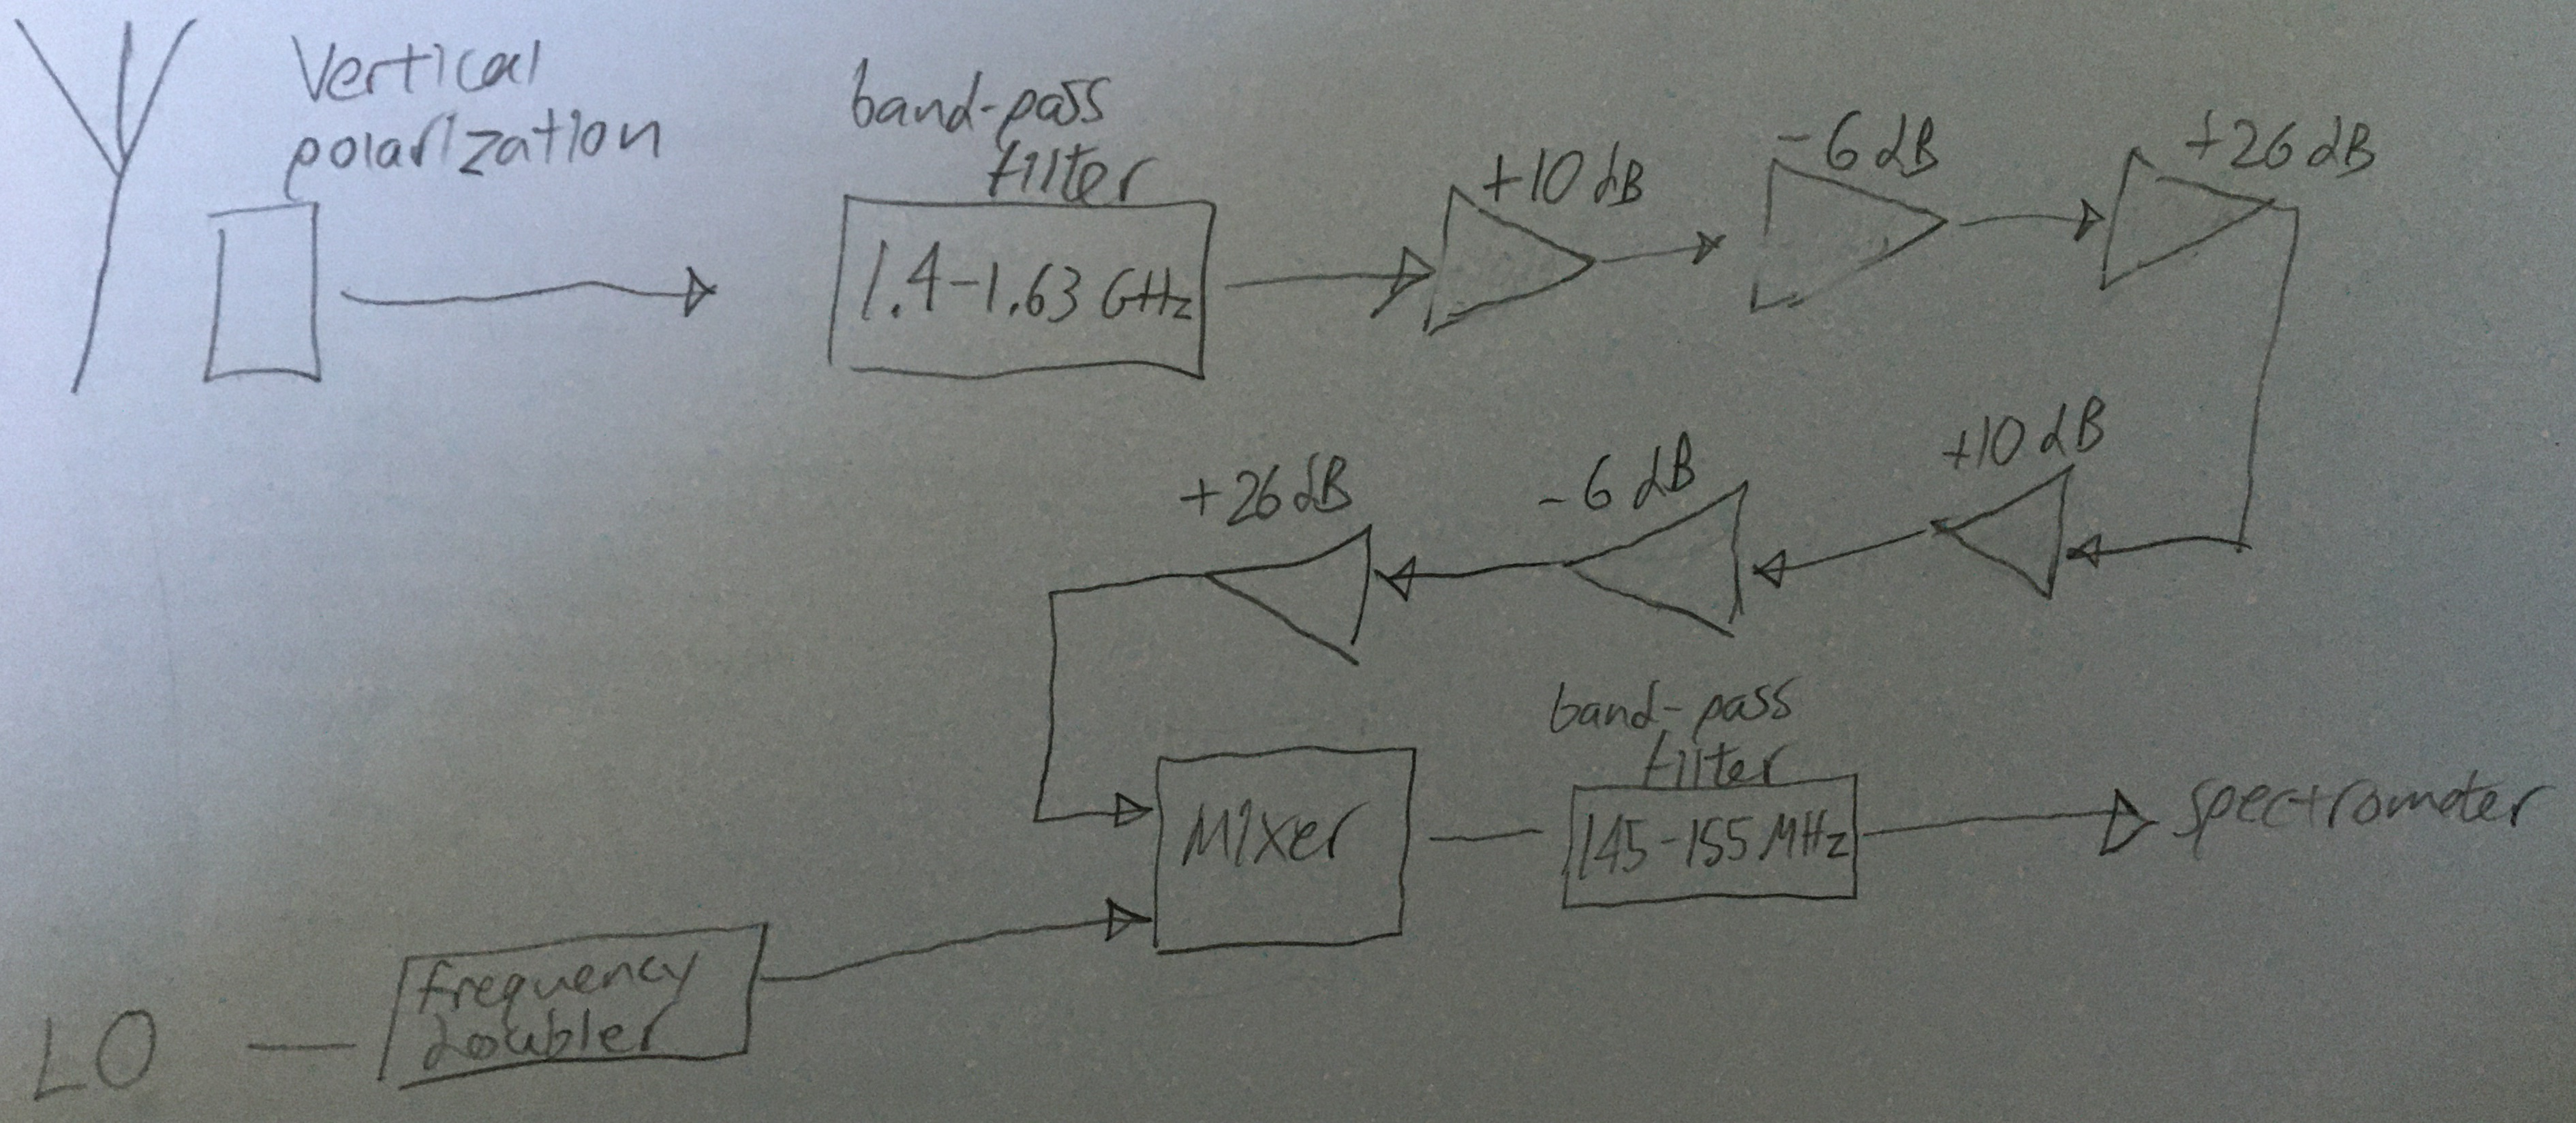
\includegraphics[width=.9\linewidth]{sig_chain}
	\caption{This is a simplification of the Leuschner signal chain, where the horizontal polarization has been ignored (we do not use those data in this report). Furthermore, we abstract-away the clock rate of the ROACH and the various stages of digitization. For our `on' LO frequency of 1270 MHz, the output spectra cover a frequency range 1415 to 1425 MHz.}
	\label{fig:sig_chain}
\end{figure}

As a demonstration of the Leuschner dish signal chain (illustrated in figure \ref{fig:sig_chain}), we show how we map a set of input signals to a final frequency axis for our plots (frequency versus brightness temperature). Since we are considering only frequency, this allows us to skip over the amplifiers and attenuators.

The initial band-pass filter ranges from 1.4 to 1.63 GHz. There is a down-converter that mixes this filtered signal with the signal from the local oscillator LO. This leads to a new frequency band (intermediate frequency IF) of 130 MHz to 360 MHz. Since we are using a real-valued mixer, we apply a band-pass filter to eliminate the sum frequencies. This filter is centered at 150 MHz and has a bandwidth of 10 MHz. Consequently, we expect the following frequency range in our outputs (which take the form of spectra in .fits files): a 10 MHz wide range beginning at 145 MHz IF (which maps to 1.415 GHz RF) and ending at 155 MHz IF (which maps to 1.425 GHz RF).

We used 1268 MHz for our second LO frequency, the `off' spectrum. This leads to an output range of 1.417 to 1.419 GHz.

% 80 K

(we used 1270 and 1268 MHz)

How we calibrate: for each value $\ell$, we take four sets of ten spectra: ...

We sample at 24 MHz (we keep 1/32 of the samples from the 768 MHz clock),->12MHz Nyquist bandwidth. so we are operating in the twelfth Nyquist window.

\section{Methods}

\quad \quad To observe the galactic plane, we have our trusty tracking script. After three labs' worth of development, it is almost correct!

We convert from galactic to topocentric coordinates using rotation matrices, as described in a previous report. How much should I include? If I describe the matrices again, that will certainly have to go in the introduction.

We probably want a basic run-down of a .fits file, but perhaps some of that can go in the introduction.

\section{Observations}

\quad \quad What would be a good $introduction$ to the data? We have hundreds of raw spectra. I am not sure how to $succinctly$ describe observations before we get into the analysis.

\section{Analysis}

\quad \quad I should explain the process of taking a spectrum to a point on our galactic plane map (Doppler shift calculations, then orthographic projection). 

\section{Conclusions}

\quad \quad We seem to have at least a couple of results! How do I estimate the uncertainty on the Leuschner dish?

\section{Acknowledgments}

\quad \quad Who did what?

Theory and background provided by Aaron Parsons. ``LAB 4: Mapping the Galactic HI Line.'' Updated April 2020.

% Can we please get a bibliography this time?

\end{document}
